\appendix

\chapter{}
\addcontentsline{toc}{chapter}{Appendix A}

\section{Diagrams}
\subsection{Use Case diagram}

\begin{figure}[H]
	\centering
	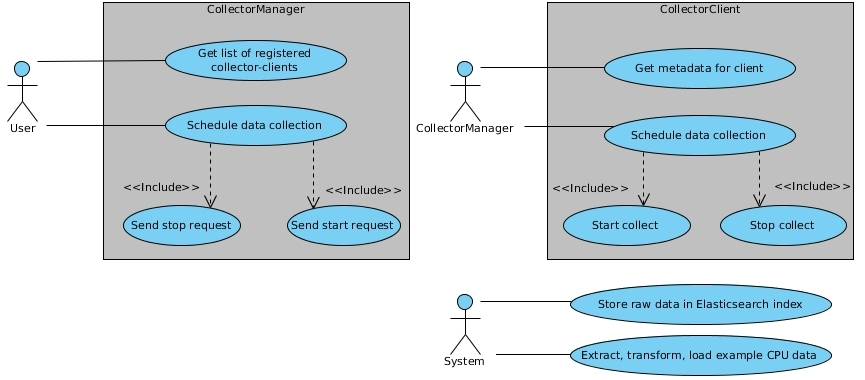
\includegraphics[width=1.0\textwidth]{../uml/usecase-collector-process.jpg}
	\caption{Use Case Diagramm}
	\label{use-case-diagram}
\end{figure}

\subsection{Class diagrams}
\begin{figure}[H]
	\centering
	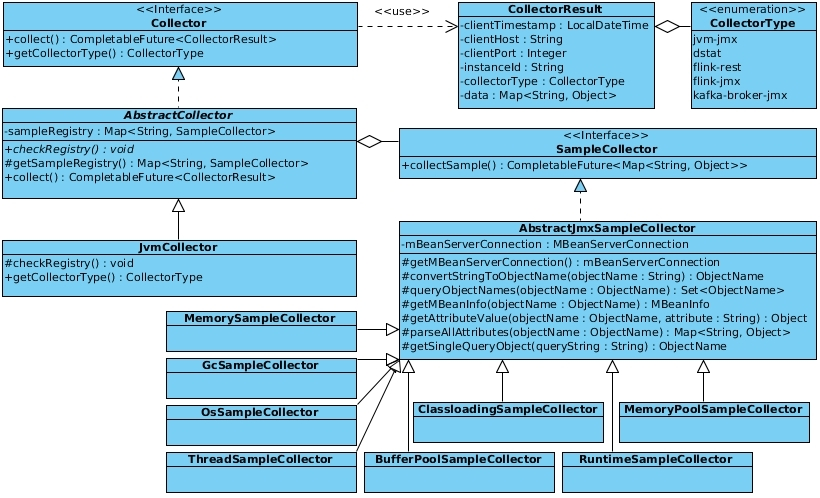
\includegraphics[width=1.0\textwidth]{../uml/class-jvm-collector.jpg}
	\caption{Class diagram 'JvmCollector'}
	\label{class-diagram-jvm-collector}
\end{figure}
\begin{figure}[H]
	\centering
	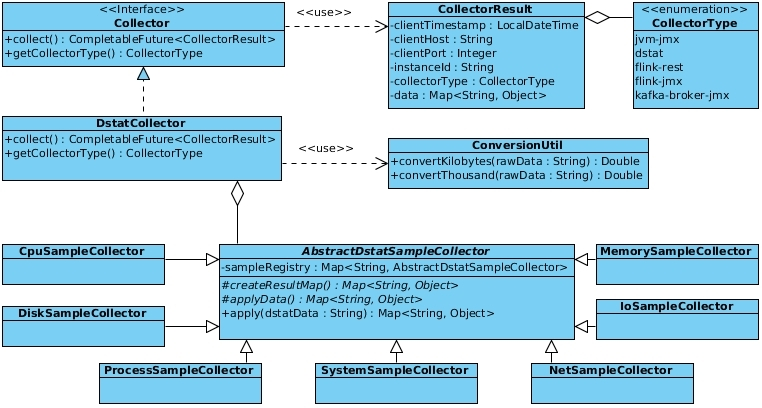
\includegraphics[width=1.0\textwidth]{../uml/class-dstat-collector.jpg}
	\caption{Class diagram 'DStatCollector'}
	\label{class-diagram-dstat-collector}
\end{figure}
\begin{figure}[H]
	\centering
	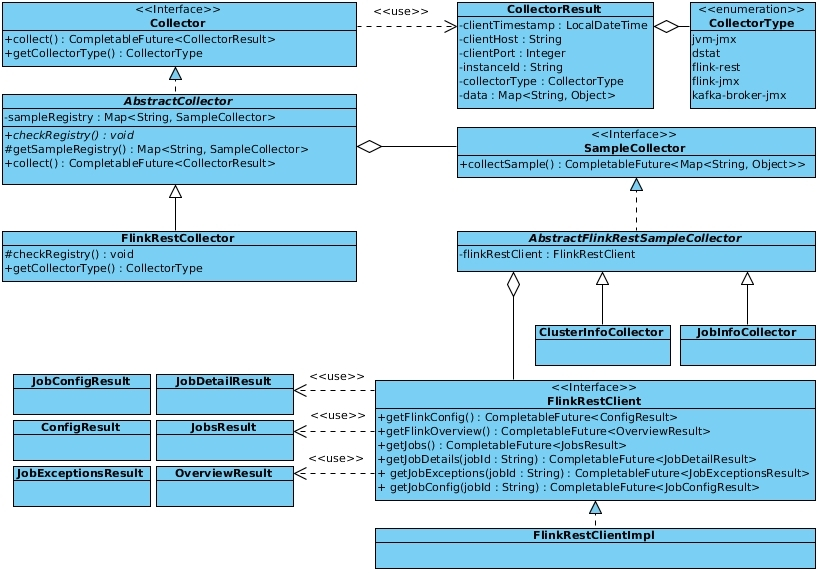
\includegraphics[width=1.0\textwidth]{../uml/class-flink-rest-collector.jpg}
	\caption{Class diagram 'FlinkRestCollector'}
	\label{class-diagram-flink-rest-collector}
\end{figure}
\begin{figure}[H]
	\centering
	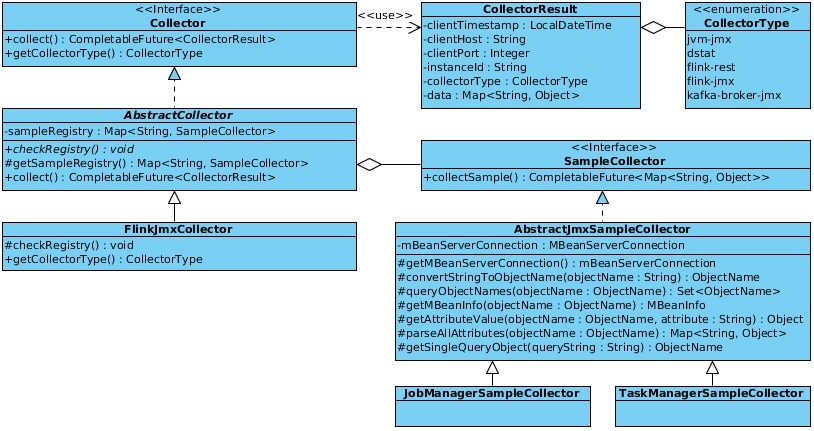
\includegraphics[width=1.0\textwidth]{../uml/class-flink-jmx-collector.jpg}
	\caption{Class diagram 'FlinkJmxCollector'}
	\label{class-diagram-flink-jmx-collector}
\end{figure}
\begin{figure}[H]
	\centering
	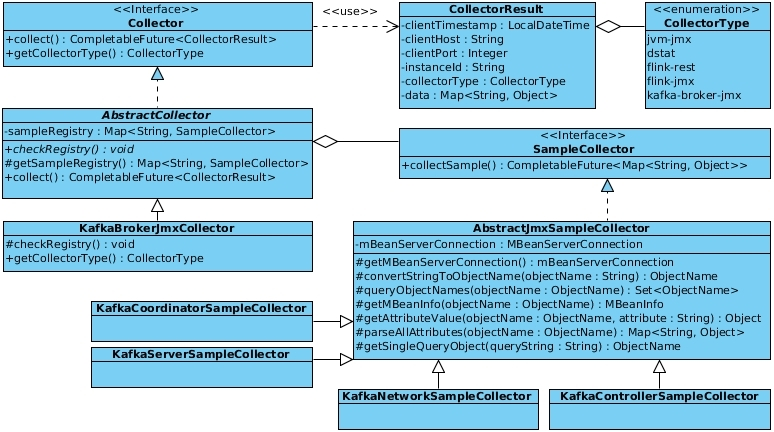
\includegraphics[width=1.0\textwidth]{../uml/class-kafka-broker-jmx-collector.jpg}
	\caption{Class diagram 'KafkaBrokerJmxCollector'}
	\label{class-diagram-kafka-broker-jmx-collector}
\end{figure}
\begin{figure}[H]
	\centering
	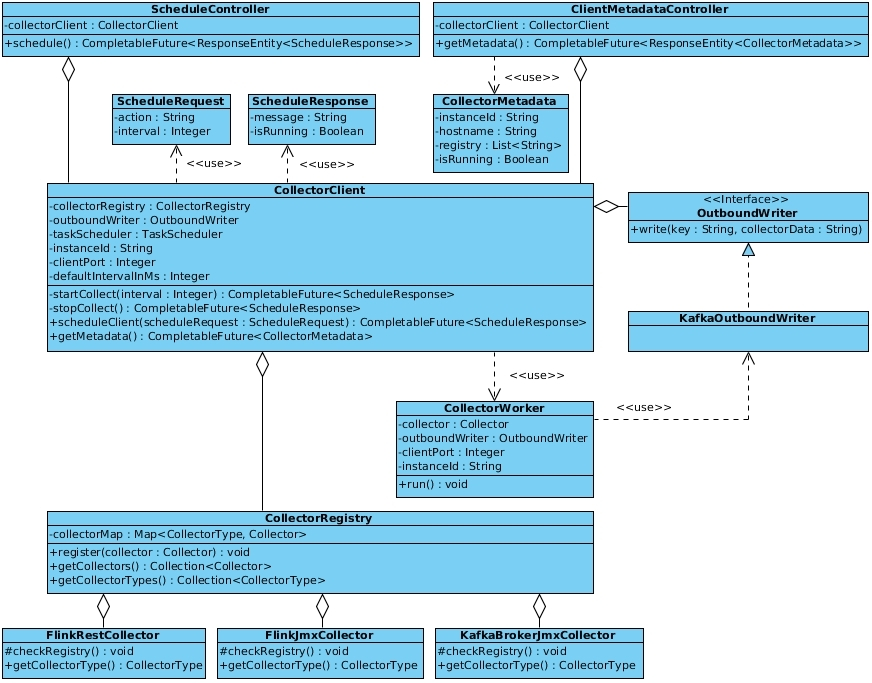
\includegraphics[width=1.0\textwidth]{../uml/class-collector-client.jpg}
	\caption{Class diagram 'CollectorClient'}
	\label{class-diagram-collector-client}
\end{figure}
\begin{figure}[H]
	\centering
	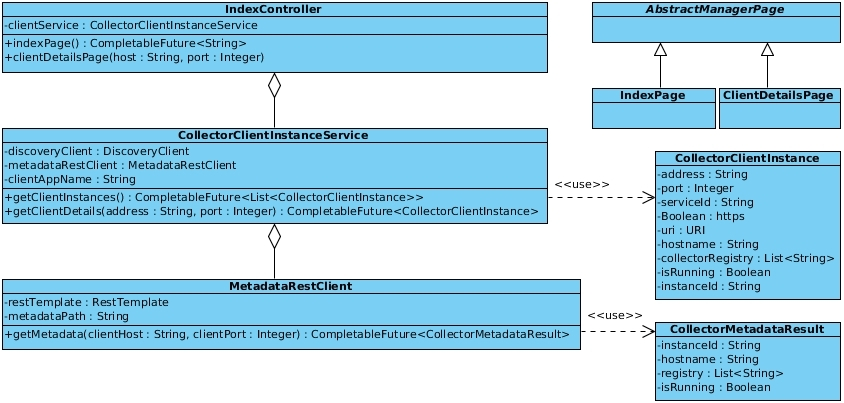
\includegraphics[width=1.0\textwidth]{../uml/class-collector-manager.jpg}
	\caption{Class diagram 'CollectorManager'}
	\label{class-diagram-collector-manager}
\end{figure}

\subsection{Sequence diagrams}
\begin{figure}[H]
	\centering
	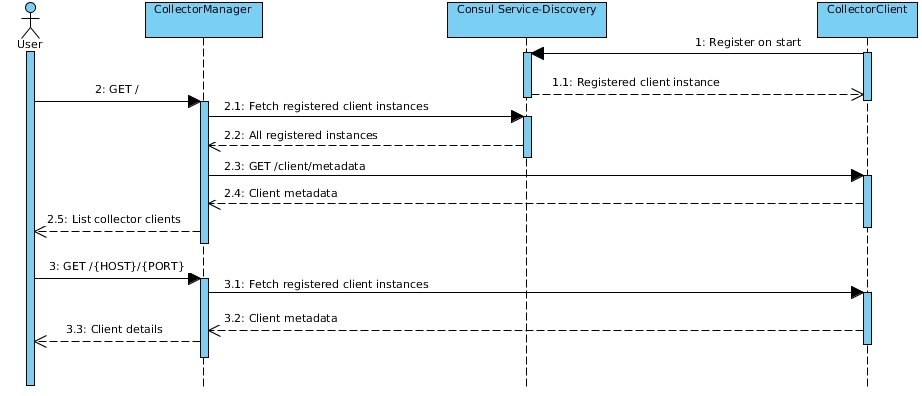
\includegraphics[width=1.0\textwidth]{../uml/sequence-discovery.jpg}
	\caption{Sequence diagram 'Client discovery'}
	\label{sequence-diagram-client-discovery}
\end{figure}
\begin{figure}[H]
	\centering
	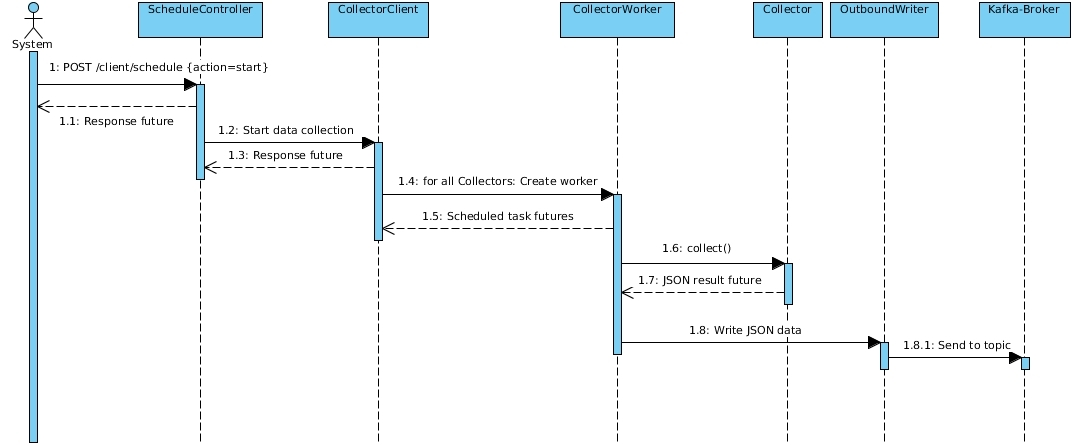
\includegraphics[width=1.0\textwidth]{../uml/sequence-scheduling.jpg}
	\caption{Sequence diagram 'Client scheduling'}
	\label{sequence-diagram-client-scheduling}
\end{figure}

\subsection{Component diagram}
\begin{figure}[H]
	\centering
	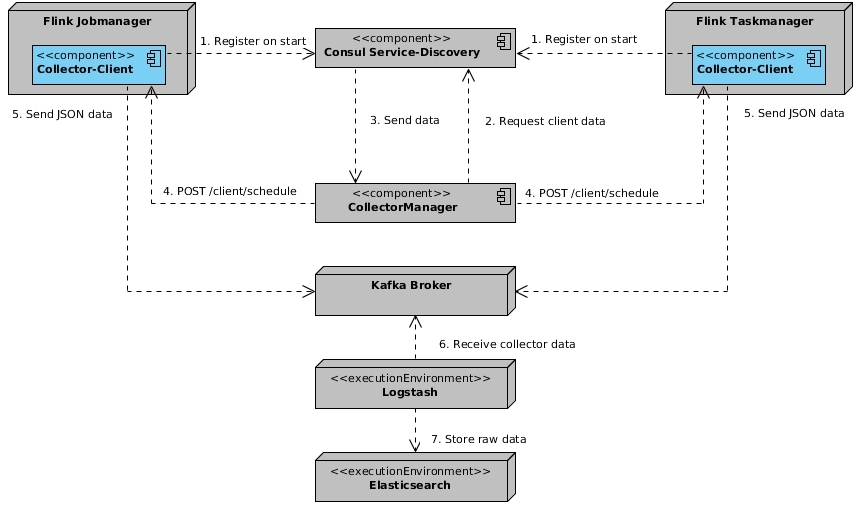
\includegraphics[width=1.0\textwidth]{../uml/component-diagram.jpg}
	\caption{Component diagram}
	\label{component-diagram}
\end{figure}

\subsection{Deployment diagram}
\begin{figure}[H]
	\centering
	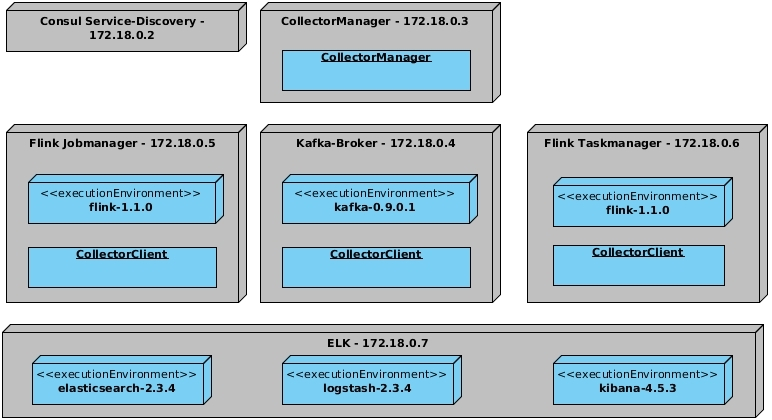
\includegraphics[width=1.0\textwidth]{../uml/deployment-diagram.jpg}
	\caption{Deployment diagram}
	\label{deployment-diagram}
\end{figure}

%\section{Collector JSON payloads}
%
%\subsection{DStatCollector}

%\begin{lstlisting}[caption={DStatCollector JSON payload}, captionpos=b, label={lst:dstatpayload}]
%{
%    "clientTimestamp": "2016-08-12T20:59:30.608",
%    "clientHost": "127.0.1.1",
%    "clientPort": 9091,
%    "instanceId": "collector-client:25ba074a0d81dd5c8e2c7b4c73152dd2",
%    "collectorType": "dstat",
%    "data": {
%        "disk": {
%            "read": 112.0,
%            "write": 436.0,
%            "utilization": 6.49,
%            "transactions": {
%                "read": 5.72,
%                "write": 8.9
%            }
%        },
%        "process": {
%            "runnable": 0.0,
%            "uninterruptible": 0.0,
%            "new": 1.4,
%            "count": 271,
%            "latency-highest-total": {
%                "name": "compiz",
%                "value": 8475.0
%            },
%            "latency-highest-avg": {
%                "name": "cat",
%                "value": 101.0
%            }
%        },
%        "memory": {
%            "usage": {
%                "used": 5548032.0,
%                "buffer": 217088.0,
%                "cache": 1626112.0,
%                "free": 695296.0
%            },
%            "process-most-expensive": {
%                "name": "java",
%                "value": 1510400.0
%            },
%            "paging": {
%                "in": 1.22265625,
%                "out": 10.8
%            },
%            "swap": {
%                "used": 312320.0,
%                "free": 7987200.0
%            },
%            "vm": {
%                "hardPageFaults": 0.5,
%                "softPageFaults": 990.0,
%                "allocated": 1476.0,
%                "free": 1500.0
%            }
%        },
%        "system": {
%            "load-avg": {
%                "1m": 1.16,
%                "5m": 1.28,
%                "15m": 1.17
%            },
%            "interrupts": 1225.0,
%            "contextSwitches": 3178.0,
%            "ipc": {
%                "messageQueue": 0.0,
%                "semaphores": 0.0,
%                "sharedMemory": 29.0
%            },
%            "unix-sockets": {
%                "datagram": 38,
%                "stream": 799,
%                "listen": 38,
%                "active": 761
%            }
%        },
%        "io": {
%            "read": 5.72,
%            "write": 8.9,
%            "process-most-expensive": {
%                "name": "upstart",
%                "pid": 3210,
%                "read": 502.0,
%                "write": 210.0,
%                "cpuPercentage": 0.0
%            },
%            "filelocks": {
%                "posix": 33.0,
%                "flock": 4.0,
%                "read": 13.0,
%                "write": 25.0
%            },
%            "filesystem": {
%                "openFiles": 13344,
%                "inodes": 48582.0
%            }
%        },
%        "cpu": {
%            "usage": [
%                {
%                    "name": "cpu0",
%                    "user": 17.0,
%                    "system": 3.3,
%                    "idle": 77.0,
%                    "wait": 2.6,
%                    "hwInterrupt": 0.0,
%                    "swInterrupt": 0.0
%                },
%                {
%                    "name": "cpu1",
%                    "user": 17.0,
%                    "system": 3.4,
%                    "idle": 77.0,
%                    "wait": 2.7,
%                    "hwInterrupt": 0.0,
%                    "swInterrupt": 0.4
%                }
%            ],
%            "process-most-expensive": {
%                "name": "java",
%                "pid": 32528,
%                "cpuPercentage": 5.8,
%                "read": 102.0,
%                "write": 272.0
%            },
%            "process-cpu-time-highest-total": {
%                "name": "Xorg",
%                "time": 40.1
%            },
%            "process-cpu-time-highest-avg": {
%                "name": "docker-compos",
%                "time": 225.0
%            }
%        },
%        "net": {
%            "traffic": [
%                {
%                    "name": "docker0",
%                    "send": 0.0,
%                    "received": 0.0
%                },
%                {
%                    "name": "wlp2s0",
%                    "send": 0.0,
%                    "received": 0.0
%                }
%            ],
%            "sockets": {
%                "total": 1.0,
%                "tcp": 19.0,
%                "udp": 8.0,
%                "raw": 0.0,
%                "ipFragments": 0.0
%            },
%            "tcp-sockets": {
%                "listen": 20.0,
%                "established": 43.0,
%                "syn": 0.0,
%                "timeWait": 5.0,
%                "close": 0.0
%            },
%            "udp": {
%                "listen": 17.0,
%                "active": 0.0
%            }
%        }
%    }
%}
%\end{lstlisting}

%\section{Screenshot}

\section{Apache Kafka MBeans version 0.9.0.2}

\begin{table}[H]
    \begin{tabular}{l}
        \textbf{JMX ObjectName} \\
        kafka.controller:type=ControllerStats,name=LeaderElectionRateAndTimeMs \\
        kafka.controller:type=ControllerStats,name=UncleanLeaderElectionsPerSec \\
        kafka.controller:type=KafkaController,name=ActiveControllerCount \\
        kafka.controller:type=KafkaController,name=OfflinePartitionsCount \\
        kafka.controller:type=KafkaController,name=PreferredReplicaImbalanceCount \\
        kafka.network:type=Processor,name=IdlePercent,networkProcessor=* \\
        kafka.server:type=socket-server-metrics,networkProcessor=* \\
        kafka.server:type=controller-channel-metrics,broker-id=* \\
        kafka.server:type=ReplicaManager,name=IsrExpandsPerSec \\
        kafka.server:type=ReplicaManager,name=IsrShrinksPerSec \\
        kafka.server:type=ReplicaManager,name=LeaderCount \\
        kafka.server:type=ReplicaManager,name=PartitionCount \\
        kafka.server:type=ReplicaManager,name=UnderReplicatedPartitions \\
        kafka.server:type=KafkaRequestHandlerPool,name=RequestHandlerAvgIdlePercent \\
        kafka.server:type=BrokerTopicMetrics,name=TotalProduceRequestsPerSec \\
        kafka.server:type=BrokerTopicMetrics,name=TotalProduceRequestsPerSec,topic=* \\
        kafka.server:type=BrokerTopicMetrics,name=TotalFetchRequestsPerSec \\
        kafka.server:type=BrokerTopicMetrics,name=TotalFetchRequestsPerSec,topic=* \\
        kafka.server:type=BrokerTopicMetrics,name=BytesInPerSec \\
        kafka.server:type=BrokerTopicMetrics,name=BytesInPerSec,topic=* \\
        kafka.server:type=BrokerTopicMetrics,name=BytesOutPerSec \\
        kafka.server:type=BrokerTopicMetrics,name=BytesOutPerSec,topic=* \\
        kafka.server:type=BrokerTopicMetrics,name=BytesRejectedPerSec \\
        kafka.server:type=BrokerTopicMetrics,name=BytesRejectedPerSec,topic=* \\
        kafka.server:type=BrokerTopicMetrics,name=FailedFetchRequestsPerSec \\
        kafka.server:type=BrokerTopicMetrics,name=FailedFetchRequestsPerSec,topic=* \\
        kafka.server:type=BrokerTopicMetrics,name=FailedProduceRequestsPerSec \\
        kafka.server:type=BrokerTopicMetrics,name=FailedProduceRequestsPerSec,topic=* \\
        kafka.server:type=BrokerTopicMetrics,name=MessagesInPerSec \\
        kafka.server:type=BrokerTopicMetrics,name=MessagesInPerSec,topic=* \\
        kafka.coordinator:type=GroupMetadataManager,name=NumGroups \\
        kafka.coordinator:type=GroupMetadataManager,name=NumOffsets \\
    \end{tabular}
    \caption{Collected Kafka MBeans}
    \label{tbl:kafka.controller}
\end{table}